\documentclass[
% -- opções da classe memoir --
12pt,				% tamanho da fonte
openright,			% capítulos começam em pág ímpar (insere página vazia caso preciso)
oneside,			% para impressão em recto e verso. Oposto a oneside
a4paper,			% tamanho do papel. 
% -- opções da classe abntex2 --
%chapter=TITLE,		% títulos de capítulos convertidos em letras maiúsculas
%section=TITLE,		% títulos de seções convertidos em letras maiúsculas
%subsection=TITLE,	% títulos de subseções convertidos em letras maiúsculas
%subsubsection=TITLE,% títulos de subsubseções convertidos em letras maiúsculas
% -- opções do pacote babel --
english,			% idioma adicional para hifenização
brazil				% o último idioma é o principal do documento
]{abntex2}

% ---
% Pacotes acrescentados
% ---
%\usepackage[portuguese, ruled, linesnumbered]{algorithm2e}
%\usepackage{algorithmic}

% ---
% Pacotes básicos 
% ---
\usepackage{lmodern}			% Usa a fonte Latin Modern			
\usepackage[T1]{fontenc}		% Selecao de codigos de fonte.
\usepackage[utf8]{inputenc}		% Codificacao do documento (conversão automática dos acentos)
\usepackage{lastpage}			% Usado pela Ficha catalográfica
\usepackage{indentfirst}		% Indenta o primeiro parágrafo de cada seção.
\usepackage{color}				% Controle das cores
\usepackage{url}				% Citar URLs
\usepackage{graphicx}			% Inclusão de gráficos
\usepackage{microtype} 			% para melhorias de justificação
\usepackage{booktabs}
\usepackage{multirow}
\usepackage[table]{xcolor}
\setlength{\aboverulesep}{0pt}
\setlength{\belowrulesep}{0pt}
\usepackage{scalefnt}
\usepackage{pdfpages}
% ---

% ---
% Pacotes adicionais, usados apenas no âmbito do Modelo Canônico do abnteX2
% ---
\usepackage{lipsum}				% para geração de dummy text
\usepackage{amssymb}			% para uso de símbolos matemáticos
% ---

% ---
% Pacotes de citações
% ---
\usepackage[brazilian,hyperpageref]{backref}	 % Paginas com as citações na bibl
\usepackage[alf]{abntex2cite}	% Citações padrão ABNT


% Pacotes adicionais Wal
\usepackage{subfig}  %para exibir figuras lado a lado
\usepackage{listings} % Para inclusao de codigos fontes
\usepackage{color}
\definecolor{mygreen}{rgb}{0,0.6,0}
\definecolor{mygray}{rgb}{0.5,0.5,0.5}
\definecolor{mymauve}{rgb}{0.58,0,0.82}
\lstset{ %
	backgroundcolor=\color{white},   % choose the background color; you must add \usepackage{color} or \usepackage{xcolor}
	basicstyle=\footnotesize,        % the size of the fonts that are used for the code
	breakatwhitespace=false,         % sets if automatic breaks should only happen at whitespace
	breaklines=true,                 % sets automatic line breaking
	captionpos=t,                    % sets the caption-position to bottom
	commentstyle=\color{mygreen},    % comment style
	deletekeywords={...},            % if you want to delete keywords from the given language
	escapeinside={\%*}{*)},          % if you want to add LaTeX within your code
	extendedchars=true,              % lets you use non-ASCII characters; for 8-bits encodings only, does not work with UTF-8
	frame=single,	                 % adds a frame around the code
	keepspaces=true,                 % keeps spaces in text, useful for keeping indentation of code (possibly needs columns=flexible)
	keywordstyle=\color{blue},       % keyword style
	language=Octave,                 % the language of the code
	otherkeywords={*,...},           % if you want to add more keywords to the set
	numbers=left,                    % where to put the line-numbers; possible values are (none, left, right)
	numbersep=5pt,                   % how far the line-numbers are from the code
	numberstyle=\tiny\color{mygray}, % the style that is used for the line-numbers
	rulecolor=\color{black},         % if not set, the frame-color may be changed on line-breaks within not-black text (e.g. comments (green here))
	showspaces=false,                % show spaces everywhere adding particular underscores; it overrides 'showstringspaces'
	showstringspaces=false,          % underline spaces within strings only
	showtabs=false,                  % show tabs within strings adding particular underscores
	stepnumber=1,                    % the step between two line-numbers. If it's 1, each line will be numbered
	stringstyle=\color{mymauve},     % string literal style
	tabsize=2,	                   	 % sets default tabsize to 2 spaces
	title=\lstname,                  % show the filename of files included with \lstinputlisting; also try caption instead of title
	numberbychapter=false
}


% --- 
% CONFIGURAÇÕES DE PACOTES
% --- 

\hyphenation{a-di-cio-nal-men-te}

% ---
% Configurações do pacote backref
% Usado sem a opção hyperpageref de backref
\renewcommand{\backrefpagesname}{Citado na(s) página(s):~}
% Texto padrão antes do número das páginas
\renewcommand{\backref}{}
% Define os textos da citação
\renewcommand*{\backrefalt}[4]{
	\ifcase #1 %
	Nenhuma citação no texto.%
	\or
	Citado na página #2.%
	\else
	Citado #1 vezes nas páginas #2.%
	\fi}%
% ---

%-----
%Adaptações do formato ABNT para UNESP
\addto\captionsbrazil{
	\renewcommand{\listfigurename}{Lista de Figuras}
	\renewcommand{\listtablename}{Lista de Tabelas}
	\renewcommand{\listadesiglasname}{Lista de Abreviaturas e Siglas}
	%\renewcommand{\folhadeaprovacaoname}{Folha de Aprovação}
	\renewcommand{\listadesimbolosname}{Lista de Símbolos}
}
%-----


% ---
% Informações de dados para CAPA e FOLHA DE ROSTO
% ---
\uppercase{\titulo{Trabalho de Pré-Processamento}}
\autor{Gabriel Luiz}
\local{Rio Claro - SP}
\data{2020}
\orientador[Professora:]{Dra. Adriane Beatriz de Souza Serapião}
\instituicao{%
	UNIVERSIDADE ESTADUAL PAULISTA
	\par
	``J\'ULIO DE MESQUITA FILHO''
	\par
	Instituto de Geociências e Ciências Exatas - IGCE
	\par
	Curso de Bacharelado em Ciências da Computação}

\tipotrabalho{Trabalho de graduação}
% O preambulo deve conter o tipo do trabalho, o objetivo, 
% o nome da instituição e a área de concentração 
\preambulo{Relatório de Trabalho de graduação da disciplina Tópicos de Aprendizado de Máquina pelo Curso de Bacharelado em Ciências da Computação do Instituto de Geociências e Ciências Exatas da Universidade Estadual Paulista “Júlio de Mesquita Filho”, Câmpus de Rio Claro. }
% ---

% ---
% Configurações de aparência do PDF final

% alterando o aspecto da cor azul
\definecolor{blue}{RGB}{41,5,195}

% informações do PDF
\makeatletter
\hypersetup{
	%pagebackref=true,
	pdftitle={\@title}, 
	pdfauthor={\@author},
	pdfsubject={\imprimirpreambulo},
	pdfcreator={regras de associação},
	pdfkeywords={java}{proposta de trabalho}{unesp}, 
	colorlinks=false,       		% false: boxed links; true: colored links
	linkcolor=blue,          	% color of internal links
	citecolor=blue,        		% color of links to bibliography
	filecolor=magenta,      		% color of file links
	urlcolor=blue,
	bookmarksdepth=4
}
\makeatother
% --- 

% --- 
% Espaçamentos entre linhas e parágrafos 
% --- 

% O tamanho do parágrafo é dado por:
\setlength{\parindent}{1.3cm}

% Controle do espaçamento entre um parágrafo e outro:
\setlength{\parskip}{0.2cm}  % tente também \onelineskip

% ---
% compila o indice
% ---
\makeindex
% ---

% ----
% Início do documento
% ----
\begin{document}
	
	% Seleciona o idioma do documento (conforme pacotes do babel)
	%\selectlanguage{english}
	\selectlanguage{brazil}
	
	% Retira espaço extra obsoleto entre as frases.
	\frenchspacing 
	
	% ----------------------------------------------------------
	% ELEMENTOS PRÉ-TEXTUAIS
	% ----------------------------------------------------------
	
	\pretextual
	
	\begin{capa}
	\begin{center}
		\Large\imprimirinstituicao
	\end{center}
	
	\begin{center}
		\vspace*{3.4cm}
		\Large GABRIEL LUIZ
		\vspace*{1.5cm}
		
		\Large \textbf{\imprimirtitulo}
		
		\vspace*{3.4cm}
		
		\noindent Professora: Dra. Adriane Beatriz de Souza Serapião
		
		\vspace*{3.4cm}
		
		{\large\imprimirlocal}
		\par
		{\large\imprimirdata}
		\vspace*{1cm}
	\end{center}
\end{capa}
	
	%\begin{folhaderosto}
	\begin{center}		
		
		\vspace*{\fill}\vspace*{\fill}
		\begin{center}
			\ABNTEXchapterfont\bfseries\Large\imprimirtitulo
		\end{center}
		\vspace*{\fill}
		
		\hspace{.45\textwidth}
		\begin{minipage}{.5\textwidth}
			\SingleSpacing
			\imprimirpreambulo
		\end{minipage}%		
		
		\vspace*{1cm}
		\begin{flushright}
			\noindent Aluno: Maicon Dall'Agnol
		\end{flushright}
		\vspace*{1cm}
		\begin{flushright}
			\noindent Professora: Dra. Adriane Beatriz de Souza Serapião
		\end{flushright}
		\vspace*{1cm}
				
				
		{\large\imprimirlocal}
		\par
		{\large\imprimirdata}
		\vspace*{1cm}
		
	\end{center}
\end{folhaderosto}
	
	%\include{errata}
	
	%\include{folhadeaprovacao}
	
	%\include{dedicatoria}
	
	%\include{agradecimentos}
	
	%\include{epigrafe}
	
	%\setlength{\absparsep}{18pt} % ajusta o espaçamento dos parágrafos do resumo
	%\include{resumo}
	
	%
%\pdfbookmark[0]{\listfigurename}{lof}
%\listoffigures*
%\cleardoublepage
% ---

% ---
% inserir lista de tabelas
% ---
%\pdfbookmark[0]{\listtablename}{lot}
%\listoftables*
%\cleardoublepage
% ---

% ---
% inserir lista de algoritmos
% ---
%\pdfbookmark[0]{Lista de Algoritmos}{loa}
%\listofalgorithms
%\cleardoublepage
% ---

% ---
% Lista de scripts
% ---
%\pdfbookmark[0]{Lista de Scripts}{loa}
%\lstlistoflistings
%\cleardoublepage

% ---
% inserir lista de abreviaturas e siglas
% ---
%\begin{siglas}
%	\item[KDD] Knowledge Discovery in Databases
%	\item[MD] Mineração da Dados
%	\item[MO] Medida Objetiva
%	\item[RA] Regra de Associação
%\end{siglas}
% ---

%\newpage
%\listofalgorithms*       % Lista de algoritmos
%\addcontentsline{toc}{section}{Lista de Algoritmos}

% ---
% inserir o sumario
% ---
\pdfbookmark[0]{\contentsname}{toc}
\tableofcontents*
\cleardoublepage
% ---

	
	% ----------------------------------------------------------
	% ELEMENTOS TEXTUAIS
	% ----------------------------------------------------------
	\textual
	
	%Capitulos
	\chapter{Proposta Trabalho Final}\label{cap_intro}

Como proposta de trabalho final para a disciplina de aprendizado de máquina é proposto desenvolver um código utilizando da linguaguem python e alguns frameworks como pandas, para realizar o processamento de imagens de flores com o intuito de classifica-las de acordo com seu tipo i.e. processar uma imagem de uma flor e dizer se é um dente de leão ou uma margaria, etc.

\section{Dataset}

Para realizar o trabalho será utilizado um dataset encontrado na basse de dados Kaggle (https://www.kaggle.com/), onde o dataset se encontra em 
(https://www.kaggle.com/alxmamaev/flowers-recognition)
 este dataset possui cinco classes de tipos de flores, que estão separados em pastas, que são:

\begin{itemize}
	\item Margaridas
	
	\item Dente de leão
	
	\item Rosas
	
	\item Girassol

	\item Tulipa.	
\end{itemize}

\section{Algoritmos}

Para este trabalho é proposto ser utilizado dois tipos de algoritmos para realizar o treinamento e classificação das imagens, sendo eles, Convolutional Neural Networks (CNN) e Random Forest e comparar os resultados obtidos para se dizer qual é o melhor algoritmo para a tarefa em questão.

\section{Convolutional Neural Networks (CNN)}

Para se realizar o processamento das imagens com o algoritmo de CNN será utilizado a biblioteca Keras, que utiliza como core o TensorFlow, ela possibilita criar e treinar modelos de aprendizado profundo, sendo fácil de usar e fácil de estender.

\section{Random Forest}

Para se realizar o processamento das imagens com o algoritmo de Random Forest será utilizado a biblioteca Skylearn que possui uma classe implementada com o algoritmo em questão.

\section{Pré Processamento}

Para o pré-processamento de ambos os algoritmos será utilizado uma biblioteca do python cv2, que permite ler as imagens, redimensionar e descrever as imagens de uma maneira que possa ser utilizada em ambos algoritmos. E também para processar os arquivos nas pastas as biblotecas glob e os

\section{Validação}

Para validar qual dos dois modelos é o melhor para o problema apresentado serão utilizadas as métricas de precisão, recall, f1-score e suporte. Onde estas metricas serão executadas para ambos os algoritmos e comparado os resultados.
	\chapter{Desenvolvimento}\label{cap_desenv}

Para o desenvolvimento das atividades inicialmente foi escolhido uma base de dados. A base a ser utilizada corresponde a dados de \textit{pacientes} que estão confirmados com o vírus covid-19 (corona víŕus).

\section{Pré-processamento e Visualização}
Na base há dados categóricos e temporais, na base em questão alguns atributos numéricos foram removidos e outros foram discretizados, também foram gerados valores float para as datas que representam cada dia em questão.

\section{Atributos}

Os atributos utilizados do dataset foram idade, sexo, data de sintomas, data de entrada no hospital, data de confirmação do virus.

O primeiro passo no pre-processamento dos dados é remover registros vazios que não possuiam alguma informação e irá atrapalhar o resultado obtido utilizando a biblioteca pandas.

\section{Idade}
Após a remoção dos valores em branco o atributo idade, é realizado uma validação de algumas idades que são reais ou seja entre 1 e 99 ou então informações em branco (NaN) são mantidas, outros valores como "4000" é removido devido a não representar nenhuma idade válida.

Depois desse processo, os valores não numericos são preenchidos com a moda da idade.

Os dados foram discretizados utilizando 3 possíveis valores, dentre eles 0 para crianças com menos de 15 anos, 1 para adultos entre 15 e 64 anos e 2 para idosos com mais de 64 anos.

\section{Sexo}
Para o sexo foi é uma normalização dos dados onde possuiam 5 possíveis valores, Female, female, Male, male, NaN, os valores que começam com a primeira letra em maiusculo devem ser alterados para ser todos minusculos.

Os valores que estão vazios devem ser preenchidos com a moda dos valores para melhor visualização dos dados.

Após este processamento deve ser discretizado os dados com 0 para male e 1 para female

\section{Datas}
As três possíveis datas do dataset selecionado serão processadas da mesma maneira, as datas estão em sua maioria no formato dd.mm.YYYY, algumas estão com o dia e o mes trocado, outras estão com informações por extenso como "final de dezembro" sem uma data especifica.

As datas que possuem informações por extensos foram removidas do dataset para nao haver informações inconsistentes dentre os dados, as datas que possuiam o mes e o dia trocadas, foram alteradas para não serem descartadas de maneira desnecessária, visto que é possível indentificar essas datas.

Após a normalização das datas, foi gerado um valor numerico que representa cada data, e os valores faltantes foram preenchidos com a média destes valores númericos representativos

\section{Visualização dos Dados}
É gerado sobre os dados a descrição deles com todos os valores utilizados para se gerar um blox-pot.

Para visualizar os dados utilizando da biblioteca seaborn, e matplotlib, foram confrontados todos os dados e valores, gerando diversos graficos, alguns podem ser uteis na visualização das informações como entrada do hospital confrontando o inicio dos sintomas ou com a data de confirmacao confrontando a entrada no hospital é possível ver a linearidade dos dados, e de que a maioria das pessoas sentem os sintomas e depois são confirmados com a doença.

Também é gerado um gráfico utilizando também da biblioteca seaborn para visualizar por exemplo que a maior quantidade de pessoas infectadas com o corona são adultos, e alguns idosos, com a minoria sendo crianças. Também é possível visualizar que a maioria das pessoas indentificadas são homens.
	%\chapter{Conclusão}\label{cap_conclu}

Aqui vai a conclusão
	
	
	% ----------------------------------------------------------
	% Finaliza a parte no bookmark do PDF
	% para que se inicie o bookmark na raiz
	% e adiciona espaço de parte no Sumário
	% ----------------------------------------------------------
	\phantompart
	
	%\chapter{Conclusão}
	
	
	% ----------------------------------------------------------
	% ELEMENTOS PÓS-TEXTUAIS
	% ----------------------------------------------------------
	\postextual
	% ----------------------------------------------------------
	
	% ----------------------------------------------------------
	% Referências bibliográficas
	% ----------------------------------------------------------
	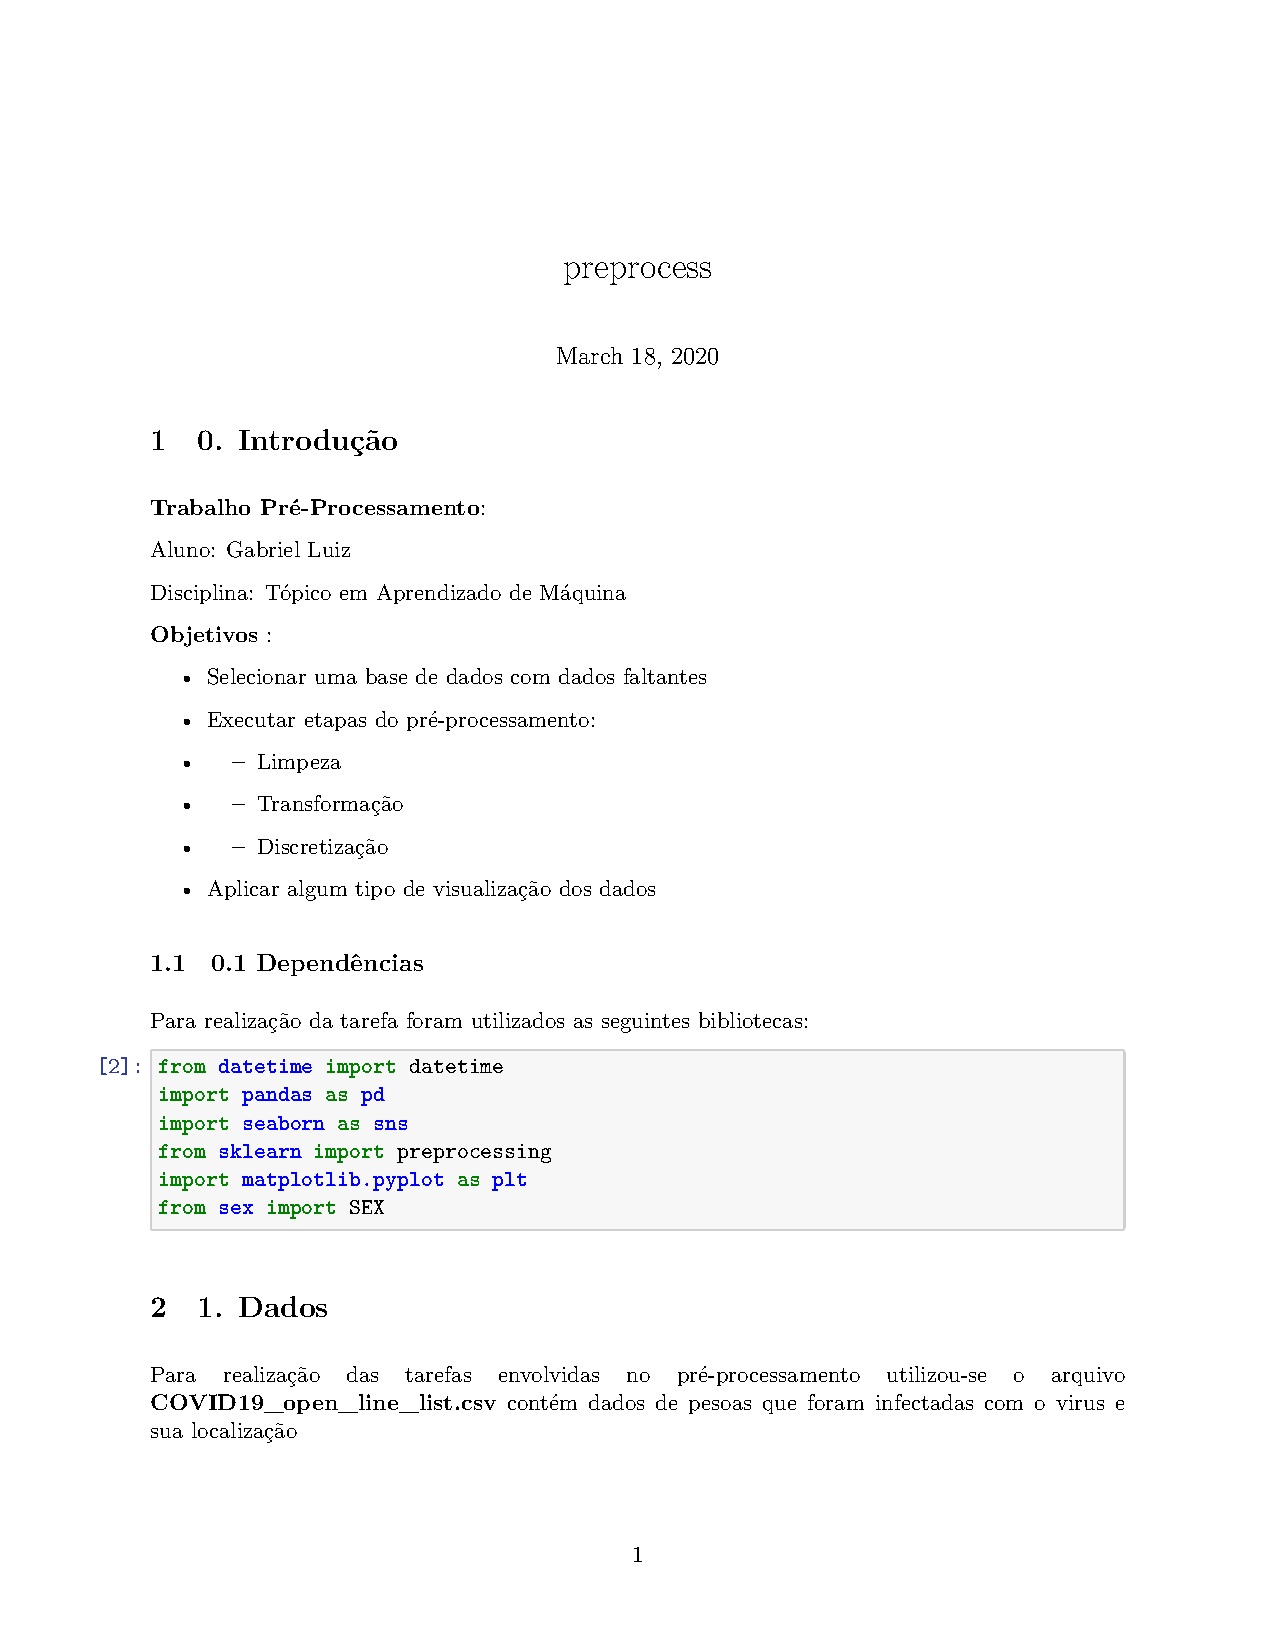
\includepdf[page=-]{preprocess}
	
	%\bibliography{references}
\end{document}
